\documentclass[conference]{IEEEtran}
\IEEEoverridecommandlockouts
\usepackage[utf8]{inputenc}
\usepackage[T1]{fontenc}
\usepackage{cite}
\usepackage{amsmath,amssymb}
\usepackage{graphicx}
\usepackage{textcomp}
\usepackage{array}
\usepackage{url}
\graphicspath{{figures/}{../../figures/}}
\begin{document}

\title{Edge-Classified Pothole and Speed-Hump Detection with a Serverless AWS IoT GIS Backend}

\author{\IEEEauthorblockN{[Author Name]}\IEEEauthorblockA{\textit{[Department], [Institution]}\\ \textit{[City], [Country]}\\ [email]}}

\maketitle

\begin{abstract}
Potholes are usually reported late and manually. We present a low-cost, end-to-end system in which an ESP32 with a three-axis accelerometer and a GPS receiver detects road events, classifies them on the device as pothole, speed hump or normal, and publishes potholes and humps with their position to a fully serverless AWS backend. An orientation-independent detector extracts the vertical dynamic acceleration and cuts a 1.5 s window around every jolt above 0.25 g; twenty shape features feed a 10-tree random forest of 17 KB. Events travel as \textasciitilde{}350-byte MQTT messages with X.509 mutual TLS to AWS IoT Core, where a rule invokes a Lambda function that stores each report in DynamoDB and folds it into a geohash cell with atomic counters, so repeated reports from any vehicle become one map marker. A second Lambda behind an HTTP API serves a Leaflet/OpenStreetMap map and GeoJSON. Under session-grouped cross-validation on 1 625 events the model reaches a macro-F1 of 0.88; on held-out real motions it labels 91 \% of drop-first events as potholes and 80 \% of lift-first events as humps. The deployed system delivered all reports from the real device to the map about 2 s after impact, within the AWS Free Tier.
\end{abstract}

\begin{IEEEkeywords}
pothole detection, edge machine learning, random forest, Internet of Things, MQTT, AWS IoT Core, serverless computing, GIS
\end{IEEEkeywords}

\section{Introduction}
Potholes damage vehicles and cause accidents, yet road agencies mostly learn about them from manual inspections and complaints. Every vehicle that hits a pothole experiences a characteristic vertical acceleration, and inexpensive MEMS accelerometers, GPS receivers and Wi-Fi microcontrollers can turn ordinary vehicles into road sensors. Managed cloud IoT services, in turn, allow reports from many vehicles to be aggregated without operating servers.

This paper describes a complete system built on these two ideas: \textbf{edge classification} of road events on a microcontroller, and a \textbf{serverless cloud backend} that aggregates the events into a shared map. Its contributions are: (i) an orientation-independent detector and a 20-feature representation that separates potholes from speed humps by the order of the vertical excursions; (ii) a 17 KB random forest selected under session-grouped cross-validation and exported to C with exact agreement; (iii) a single-template AWS backend (IoT Core, Lambda, DynamoDB, API Gateway) with crowd aggregation and open GeoJSON output; and (iv) an end-to-end deployment verified with the real device.

\section{Related Work}
Pothole Patrol \cite{r1} mounted accelerometers and GPS in taxis, detected potholes with a cascade of tuned filters and clustered reports across vehicles to remove false positives; our aggregation follows the same principle. Nericell \cite{r2} used smartphones and introduced virtual re-orientation using the gravity vector. Mednis et al. \cite{r3} compared threshold detectors on Android phones and noted their dependence on vehicle and mounting. Tree ensembles \cite{r4,r5} trained with scikit-learn \cite{r6} replace fixed thresholds with learned decisions while remaining small enough for microcontrollers. Edge computing \cite{r7} motivates classifying on the device; serverless computing \cite{r8}, MQTT \cite{r9} and GeoJSON \cite{r10} provide the cloud and GIS building blocks.

\section{System Architecture}
Fig.~\ref{fig:arch} shows the system. The device samples a three-axis accelerometer (MPU-6050 or ADXL345, $\pm$8 g, 100 Hz, I2C) and a u-blox NEO-7M GPS (5 Hz, UART) on an ESP32. Only classified events leave the device: raw data would be about 1 KB/s per vehicle, whereas one event is a \textasciitilde{}350-byte JSON message.

\begin{figure}[t]
\centering
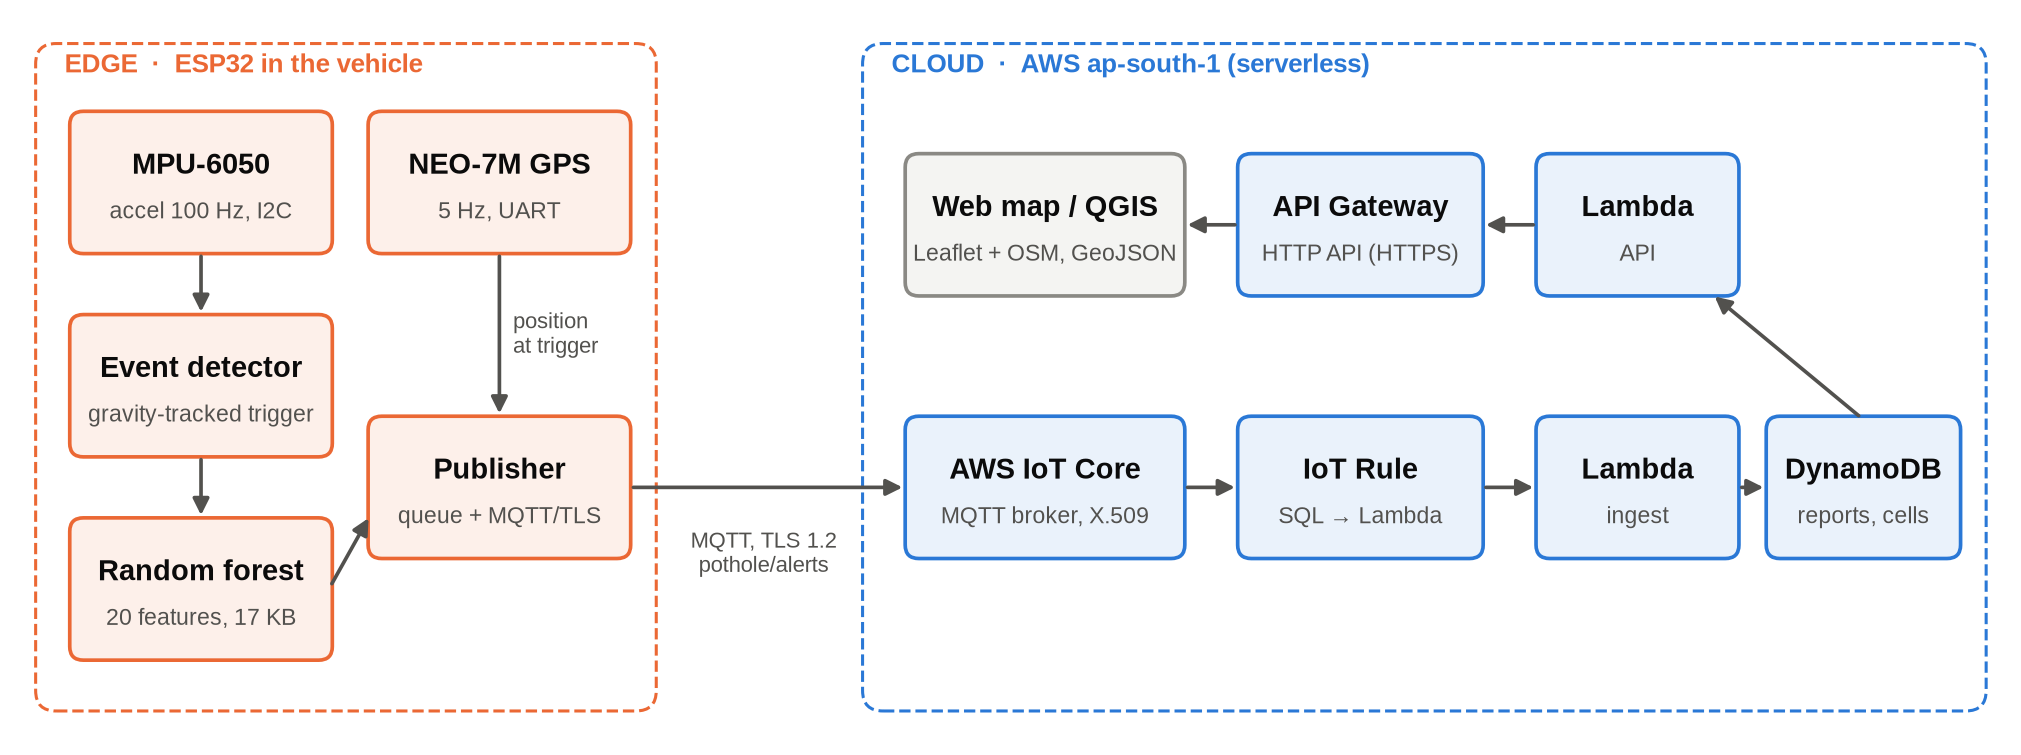
\includegraphics[width=\columnwidth]{fig_architecture.png}
\caption{System architecture: classification on the ESP32, serverless backend in AWS ap-south-1.}
\label{fig:arch}
\end{figure}

\subsection{Edge Device}
Four FreeRTOS tasks run on the ESP32: a high-priority sensor task on core 1 (detection and inference), a publish task with a 32-event queue that survives connectivity loss, a GPS parser and a status LED. The GPS state is copied at the trigger instant, so a report carries the position where the wheel hit. Potholes and humps with a class probability of at least 0.6 are published with QoS 1 to topic \texttt{pothole/alerts} over TLS 1.2 on port 8883, authenticated by a per-device X.509 certificate.

\subsection{Cloud Backend}
All cloud resources are defined in one AWS SAM template and deployed as a CloudFormation stack (Table~\ref{tab:svc}). An IoT rule \texttt{SELECT *, timestamp() AS received\_ms, clientid() AS clientid FROM 'pothole/alerts'} invokes the ingest Lambda for every message. The device policy permits only \texttt{iot:Connect} and \texttt{iot:Publish} to that topic.

\begin{table}[t]
\caption{AWS services used}
\label{tab:svc}
\centering
\footnotesize
\begin{tabular}{l p{5.4cm}}
\hline
\textbf{Service} & \textbf{Role} \\
\hline
IoT Core & MQTT broker; thing, X.509 certificate, publish-only policy; topic rule \\
Lambda ($\times$2) & ingest: validate, store, aggregate; API: map page and GeoJSON (Python 3.12, arm64) \\
DynamoDB & single on-demand table: raw reports (90-day TTL) and map cells \\
API Gateway & HTTP API: GET / and GET /potholes \\
CloudFormation, S3, CloudWatch, IAM & IaC stack, artefacts, logs, least-privilege roles \\
\hline
\end{tabular}
\end{table}

\subsection{Aggregation and Map}
A report is mapped if its event is POTHOLE or SPEED\_HUMP, its coordinates are valid and its HDOP is at most 5; otherwise it is stored with the reason. Mapped reports are folded into a geohash-8 cell (about 38 m $\times$ 19 m) keyed \texttt{CELL\#\textless{}geohash\textgreater{}} / \texttt{TYPE\#\textless{}event\textgreater{}} with an atomic \texttt{ADD} of the count and of the latitude, longitude and confidence sums, so concurrent vehicles need no read-modify-write. At query time cells of the same type within 15 m are merged and returned as a GeoJSON FeatureCollection. The report count acts as confidence: a pothole confirmed by several vehicles becomes a larger marker on a Leaflet/OpenStreetMap map, and the same feed loads into QGIS.

\section{Event Detection and Classification}
\subsection{Detector}
Each sample \textbf{a} updates a low-pass gravity estimate \textbf{g} ($\tau$ $\approx$ 1 s, ten times slower during events). The vertical dynamic acceleration is \emph{v = a$\cdot$$\hat{g}$ $-$ \textbar{}g\textbar{}} and the horizontal one \emph{h = \textbar{}a $-$ g $-$ v$\hat{g}$\textbar{}}, so any mounting angle works. When \textbar{}v\textbar{} \textgreater{} 0.25 g a 150-sample window (0.5 s before, 1.0 s after the trigger) is captured, followed by a 0.3 s cooldown. Flat road never triggers, which removes most false positives and keeps the CPU idle. Fig.~\ref{fig:sig} shows why the order of the excursions matters.

\begin{figure}[t]
\centering
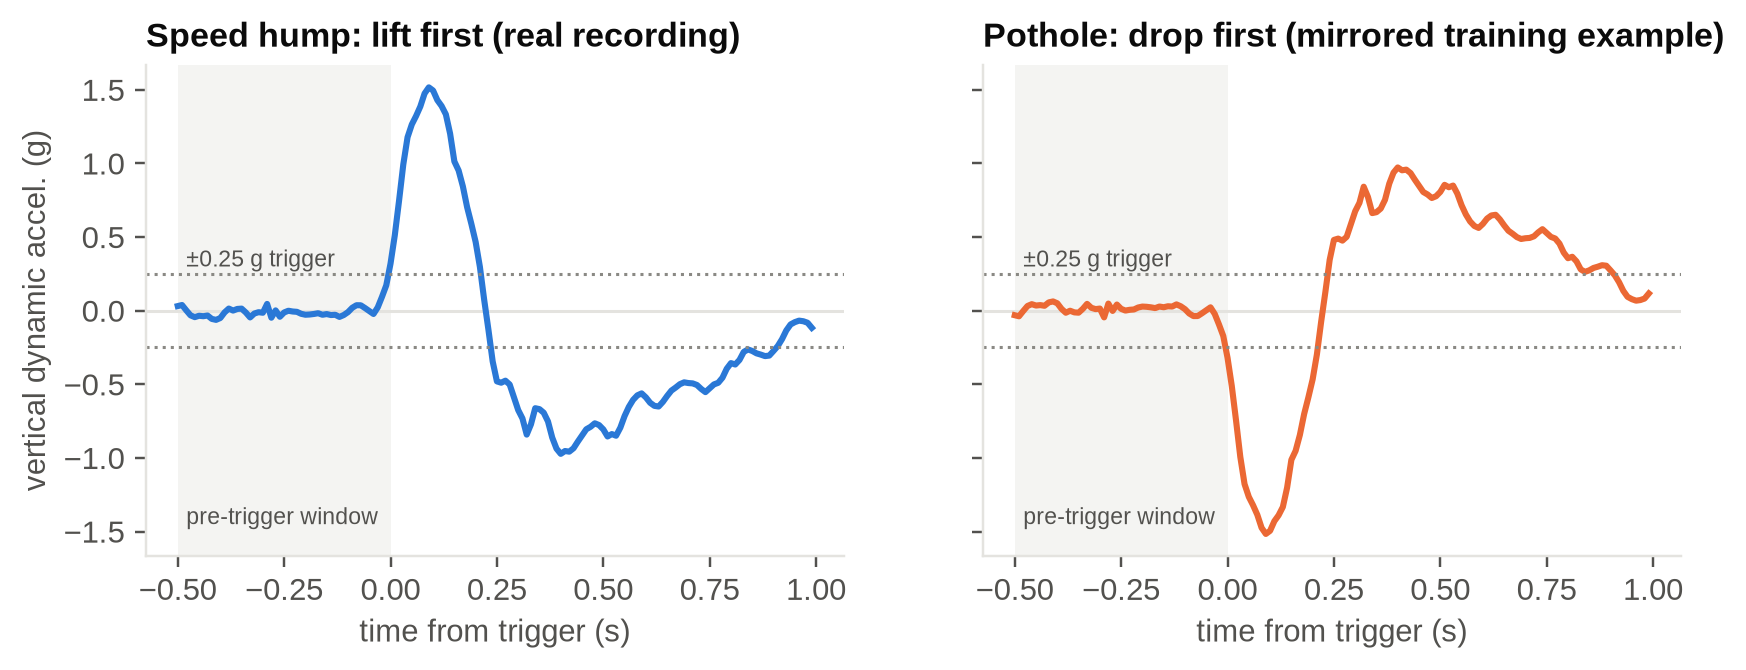
\includegraphics[width=\columnwidth]{fig_signal.png}
\caption{Vertical dynamic acceleration around the trigger: a real speed hump (lift first) and the mirrored pothole example (drop first).}
\label{fig:sig}
\end{figure}

\subsection{Features}
Twenty features are computed from v and h: magnitude (max, min, peak-to-peak, standard deviation, mean of v), \textbf{order} (sign of the first large excursion; time of maximum minus time of minimum), duration above threshold, sharpness (maximum jerk, high-frequency energy ratio, crest factor, kurtosis), roll (max and standard deviation of h, h/v ratio), zero-crossing rate, pre-event roughness, signed areas and skewness. The C implementation is compiled both into the firmware and into a host library called from Python via ctypes, so training features are bit-identical to the device's.

\subsection{Data and Training}
Training data combine (i) a quarter-car simulator with random vehicles, speeds, mounting angles and ISO 8608 road roughness \cite{r11}; (ii) real bench recordings with the MPU-6050; and (iii) augmentations of the real events (rotation, amplitude 0.7--1.35$\times$, time stretch 0.85--1.2$\times$, noise). Real events are filtered by their defining shape before augmentation; lacking clean real potholes, pothole examples are mirrored real humps plus parametric drop--jolt events. The final set has 1 625 events (398 normal, 660 hump, 567 pothole) from 58 sessions. Seventeen trees, random forests and extra-trees were scored by macro-F1 under five-fold \textbf{session-grouped} cross-validation, and the smallest model within 0.01 of the best was selected. The forest is exported as flat C arrays with uint8 leaf probabilities; the exporter checks agreement with scikit-learn on every event.

\section{Results}
\subsection{Classification}
With axis statistics (minimum, maximum, mean per axis) the macro-F1 on simulated drives was 0.20--0.28; the shape features raise it to 0.84 (tree) and 0.92 (forest). Among all candidates (Fig.~\ref{fig:models}), a 25-tree forest scored 0.881 with 3 769 nodes, while the selected 10-tree depth-8 forest scored 0.877 with 1 452 nodes (\textasciitilde{}17 KB flash, 100 \% C/Python agreement). Table~\ref{tab:perclass} gives its per-class results and Fig.~\ref{fig:cm} its confusion matrix. The most important features are the extreme-order feature (0.187) and the first-peak sign (0.130). On real motions held out from all training and augmentation, 91 \% of drop-first motions were classified as potholes and 80 \% of lift-first motions as speed humps.

\begin{figure}[t]
\centering
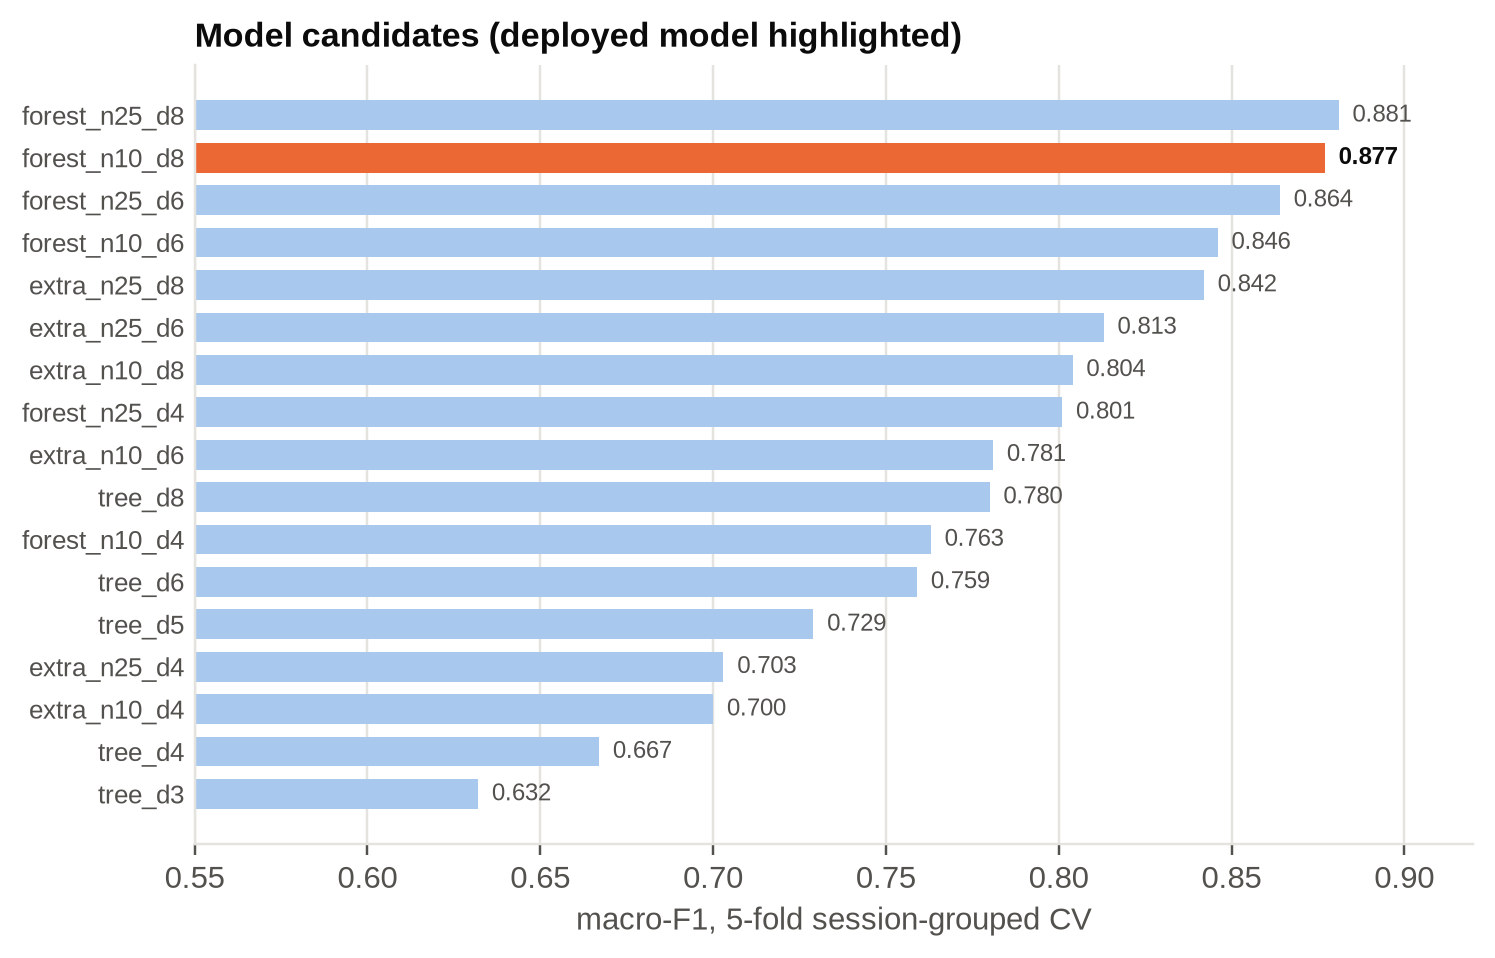
\includegraphics[width=\columnwidth]{fig_models.png}
\caption{Session-grouped cross-validated macro-F1 of the 17 candidates; the deployed model is highlighted.}
\label{fig:models}
\end{figure}

\begin{table}[t]
\caption{Per-class results of the deployed forest (5-fold grouped CV)}
\label{tab:perclass}
\centering
\footnotesize
\begin{tabular}{lcccc}
\hline
\textbf{Class} & \textbf{Precision} & \textbf{Recall} & \textbf{F1} & \textbf{Support} \\
\hline
normal & 0.83 & 0.84 & 0.83 & 398 \\
speed hump & 0.91 & 0.89 & 0.90 & 660 \\
pothole & 0.89 & 0.91 & 0.90 & 567 \\
macro avg. & 0.88 & 0.88 & 0.88 & 1 625 \\
\hline
\end{tabular}
\end{table}

\begin{figure}[t]
\centering
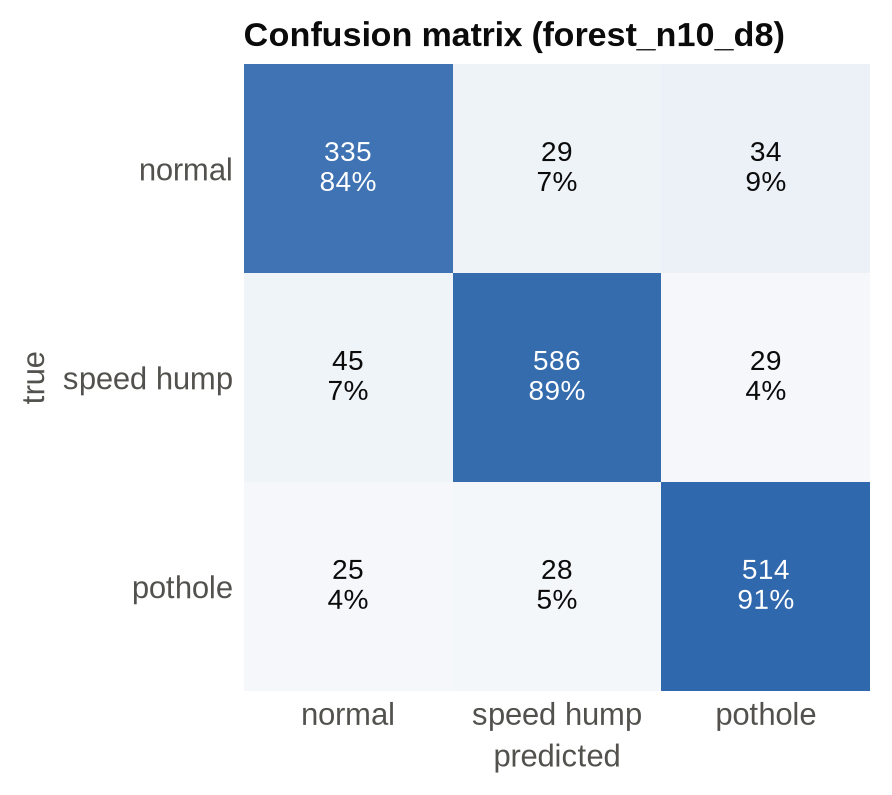
\includegraphics[width=\columnwidth]{fig_confusion.png}
\caption{Confusion matrix of the deployed forest.}
\label{fig:cm}
\end{figure}

\subsection{End-to-End Deployment}
The backend was deployed in AWS ap-south-1 and the device was provisioned with its own certificate. With a phone hotspot and a GPS fix of 7--8 satellites (HDOP 0.9--2.4) the device connected to IoT Core within 14 s of boot. Table~\ref{tab:verif} summarises the verification: all six reports produced by desk motions (three potholes, three humps) were stored and mapped, and the three potholes, a few metres apart, were merged into one marker with three reports. The trigger-to-database latency is about 1.5--2 s, dominated by the 1 s post-trigger window, and the running cost lies within the AWS Free Tier.

\begin{table}[t]
\caption{Verification of the deployed system}
\label{tab:verif}
\centering
\footnotesize
\begin{tabular}{ll}
\hline
\textbf{Test} & \textbf{Result} \\
\hline
Lambda logic, offline & passed \\
SAM template lint & valid \\
Synthetic publish (AWS CLI) & marker in GeoJSON \\
Real device, real GPS & 6/6 reports mapped \\
Aggregation & 3 potholes $\rightarrow$ 1 marker \\
Latency trigger $\rightarrow$ DB & $\approx$ 1.5--2 s \\
\hline
\end{tabular}
\end{table}

\section{Discussion and Limitations}
The order of the vertical excursions is the decisive cue, which explains both the large gain over axis statistics and the robustness to mounting. The main limitation is the data: the model has seen simulated vehicle dynamics and hand motions only, and real potholes are represented by mirrored humps. GPS error of a few metres is comparable to pothole size, so the 15 m merge radius may join neighbouring potholes. The map is public and read-only and has no mechanism yet to mark repairs.

\section{Conclusion}
An ESP32 running a 17 KB random forest separates potholes from speed humps with a cross-validated macro-F1 of 0.88, and a serverless AWS backend defined in a single template turns its MQTT reports into a crowd-aggregated GIS map at negligible cost. Future work is to collect real road data and retrain, to add repair tracking and report ageing, and to distribute updated models through device shadows and OTA updates.

\begin{thebibliography}{00}
\bibitem{r1} J. Eriksson, L. Girod, B. Hull, R. Newton, S. Madden, and H. Balakrishnan, ``The Pothole Patrol: Using a mobile sensor network for road surface monitoring,'' in \emph{Proc. MobiSys}, 2008, pp. 29--39.
\bibitem{r2} P. Mohan, V. N. Padmanabhan, and R. Ramjee, ``Nericell: Rich monitoring of road and traffic conditions using mobile smartphones,'' in \emph{Proc. ACM SenSys}, 2008, pp. 323--336.
\bibitem{r3} A. Mednis, G. Strazdins, R. Zviedris, G. Kanonirs, and L. Selavo, ``Real time pothole detection using Android smartphones with accelerometers,'' in \emph{Proc. DCOSS}, 2011, pp. 1--6.
\bibitem{r4} L. Breiman, ``Random forests,'' \emph{Mach. Learn.}, vol. 45, no. 1, pp. 5--32, 2001.
\bibitem{r5} P. Geurts, D. Ernst, and L. Wehenkel, ``Extremely randomized trees,'' \emph{Mach. Learn.}, vol. 63, no. 1, pp. 3--42, 2006.
\bibitem{r6} F. Pedregosa \emph{et al.}, ``Scikit-learn: Machine learning in Python,'' \emph{J. Mach. Learn. Res.}, vol. 12, pp. 2825--2830, 2011.
\bibitem{r7} W. Shi, J. Cao, Q. Zhang, Y. Li, and L. Xu, ``Edge computing: Vision and challenges,'' \emph{IEEE Internet Things J.}, vol. 3, no. 5, pp. 637--646, 2016.
\bibitem{r8} E. Jonas \emph{et al.}, ``Cloud programming simplified: A Berkeley view on serverless computing,'' UC Berkeley, Tech. Rep. UCB/EECS-2019-3, 2019.
\bibitem{r9} OASIS, ``MQTT version 3.1.1,'' OASIS Standard, 2014.
\bibitem{r10} H. Butler, M. Daly, A. Doyle, S. Gillies, S. Hagen, and T. Schaub, ``The GeoJSON format,'' IETF RFC 7946, 2016.
\bibitem{r11} ISO 8608:2016, \emph{Mechanical vibration --- Road surface profiles --- Reporting of measured data}, ISO, 2016.
\bibitem{r12} Amazon Web Services, ``AWS IoT Core developer guide.'' [Online]. Available: \url{https://docs.aws.amazon.com/iot/}
\end{thebibliography}

\end{document}
